%=== CHAPTER TWO (2) ===
%=== Literature Review ===

\chapter{Literature Review}
\label{cha:literature}
\begin{spacing}{1.5}
\setlength{\parskip}{0.3in}

\section{Introduction}

Then comes the main part of your work. To lay the ground, there should first be a chapter on what has been done before on the problem - a Literature Review. This is an important section because it shows that you do not narrowly focus only on what you do, but are aware of the
related work elsewhere, some of which might be instructive to your solving the problem. It can also explain why you are taking the direction you do.

\section{An Overview}
\label{sec:LR_overview}

In the past few years, the lane detection method have been developed from classical ones to novel deep-learning based ones. In this section, I will give a brief review of the classical lane detection methods proposed, and also give a brief overview of the developments in the field of object detection.

\subsection{Classical Lane Detection}

There are several ways to get the information for lane detection and prediction usage, such as Monocular vision, stereo, LIDAR, inertial measurement unit (IMU) combined with information obtained from global positioning system (GPS) and high resolution digital maps. \cite{hillel2014recent}. In this work I focus on Monocular vision (Single camera).

In previous work, researchers found relation between wheeling and gaze direction when driving. Human employs the distant region to estimate the road curvature \cite{land1995parts}. Also, the gaze direction relies on the 'tangent point' on the inside of each curve when driving on curvature of the road ahead \cite{land1994we}. This gives possible to utilize the unseen vanishing point in lane prediction.

\subsection{Deep-learning based Lane Detection}

Lane and road marking detection tasks are within the scope of object detection, so algorithms popular in object detection have been implemented in lane detection \cite{tang2020review}. 

Recent years, with the DCNN like AlexNet \cite{krizhevsky2012imagenet} being brought up, deep learning has been driving significant progress in the object detection area. Later RCNN and its variants \cite{girshick2014rich, girshick2015fast, ren2015faster} integrates CNN with the region proposal selective search; GoogLeNet \cite{szegedy2015going} and VGGNet \cite{simonyan2014very} gained improvement with deeper encoder. With the network going deeper, computational efficiency becomes the main problem. More powerful network architectures such as ResNets \cite{he2016deep}, DenseNets \cite{huang2017densely} and Inception \cite{ioffe2015batch} have been proposed, which combine path blocks to reduce the number of parameters while improving the accuracy. Most recently, DETR \cite{carion2020end} combined the CNN with transformer architecture, taking the object detection problem as a set-set mapping and achieved promising results on big-object detection.

Lanes are thin and small objects, thus general methods sometimes work bad \cite{tang2020review}. There are some researches featured in picking out small items. U-Net \cite{ronneberger2015unet} extracts the feature map from encoding path and attach it with the decoding path, by which method the network can keep context for local features.

Efforts to use the neural network in lane detection tasks have also been proved solid. Work \cite{borji2016vanishing} first used the CNN structure to predict the vanishing point, and VPGNet \cite{lee2017vpgnet} employed vanishing point information by multi-task method to enhance the prediction of the lanes.

\section{Neural Network Basis}

Neural Network is the most distinguish deep learning architecture based on Neural units recent years. Compared with conventional machine learning and human-designed mathematical classification algorithms, deep learning on the Neural Network have many advantages. In this section, I will give the theoretical basis of the Neural Networks, and also explain how it works by introducing the back propagation mechanism.

\subsection{Machine Learning}

Compared with specific mathematical equations designed for different kinds of problems, the conventional machine learning are based on \textit{experience}. \textit{Experience} here means that: the machine learning computational models can learn the features from a given data set (learn the \textit{experience} from input), and do prediction or classification based on the that \textit{experience} for any inputs, whether have seen or unseen before.~\cite{mohri2018foundations}.

The process of learning the features can be seen as a clustering operation. Each input data can be mapped into a $n$-dimension vector, and each vector can be viewed as a point in the $n$-dimension hyperspace. \autoref{fig:2dcluster} and \autoref{fig:3dcluster} shows the $2D$ and $3D$ clustering process. Clustering is to group data points into different clusters in the hyperspace, and draw the hyperplane between such clusters. This hyperplane is the interface between classes. For example, in figure \autoref{fig:2dcluster}, 2 groups of data were divided by a linear line, and in figure \autoref{fig:3dcluster}, 2 groups of data were divided by a non-linear curved surface.

\begin{figure}[ht]
\centering
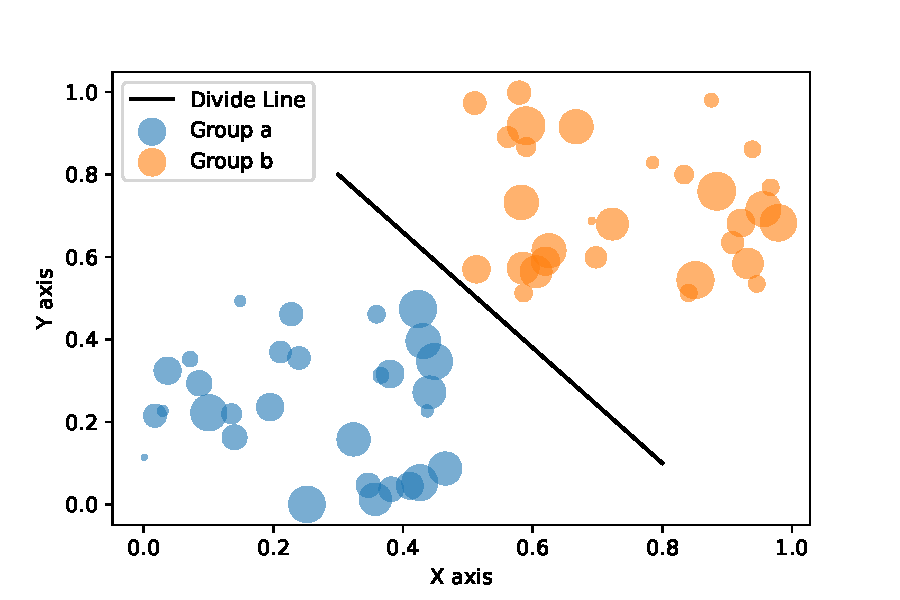
\includegraphics[width=0.99\textwidth, fbox]{Chapter2/2dcluster.pdf}
\caption{$2D$ Clustering}
\label{fig:2dcluster} 
\end{figure}

% \begin{figure}[ht]
% \centering
% \fbox{
% \includesvg[width=0.97\textwidth]{Chapter2/3dcluster.svg}
% }
% \caption{$2D$ Clustering}
% % \label{fig:2dcluster} 
% \end{figure}

\begin{figure}[ht]
\centering
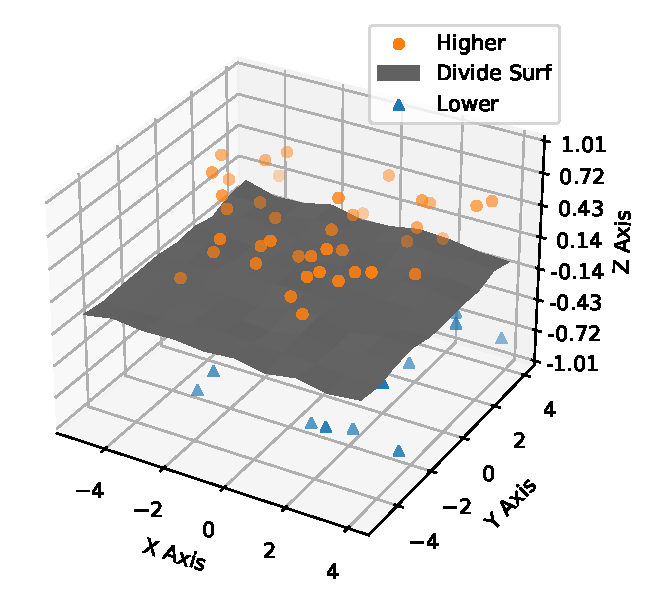
\includegraphics[width=0.6\textwidth, fbox]{Chapter2/3dcluster.pdf}
\caption{$3D$ Clustering}
\label{fig:3dcluster} 
\end{figure}

Above mentioned examples only calculate linear or non-linear division between two classes, but normally in real world applications, what needed are not limited to binary classification but usually multi-classification. In the machine learning, there are two solutions on multi-classification problem: 

1) \textit{Uncombined algorithms} will treat the multi-classification as a whole and finish training in only one phase, such as $N$-class SVM, decision trees. 

2) \textit{Aggregated algorithms} will split $N$ class classification into many binary classification, thus need multiple training phase. There are two types of aggregated algorithms: a) \textit{One-versus-one} calculate boundaries for every pair of classes, thus for $N$ class, it needs $N!=N*(N-1)*...*2*1$ calculations, as shown in \autoref{fig:121}. b) \textit{One-versus-others} calculate the boundary between the target class and all other data, thus for $N$ class, it needs to calculate $N$ boundaries, as shown in \autoref{fig:12all}. 

\begin{figure}[th]
    \centering
    \begin{subfigure}[b]{0.49\textwidth}
        \centering
        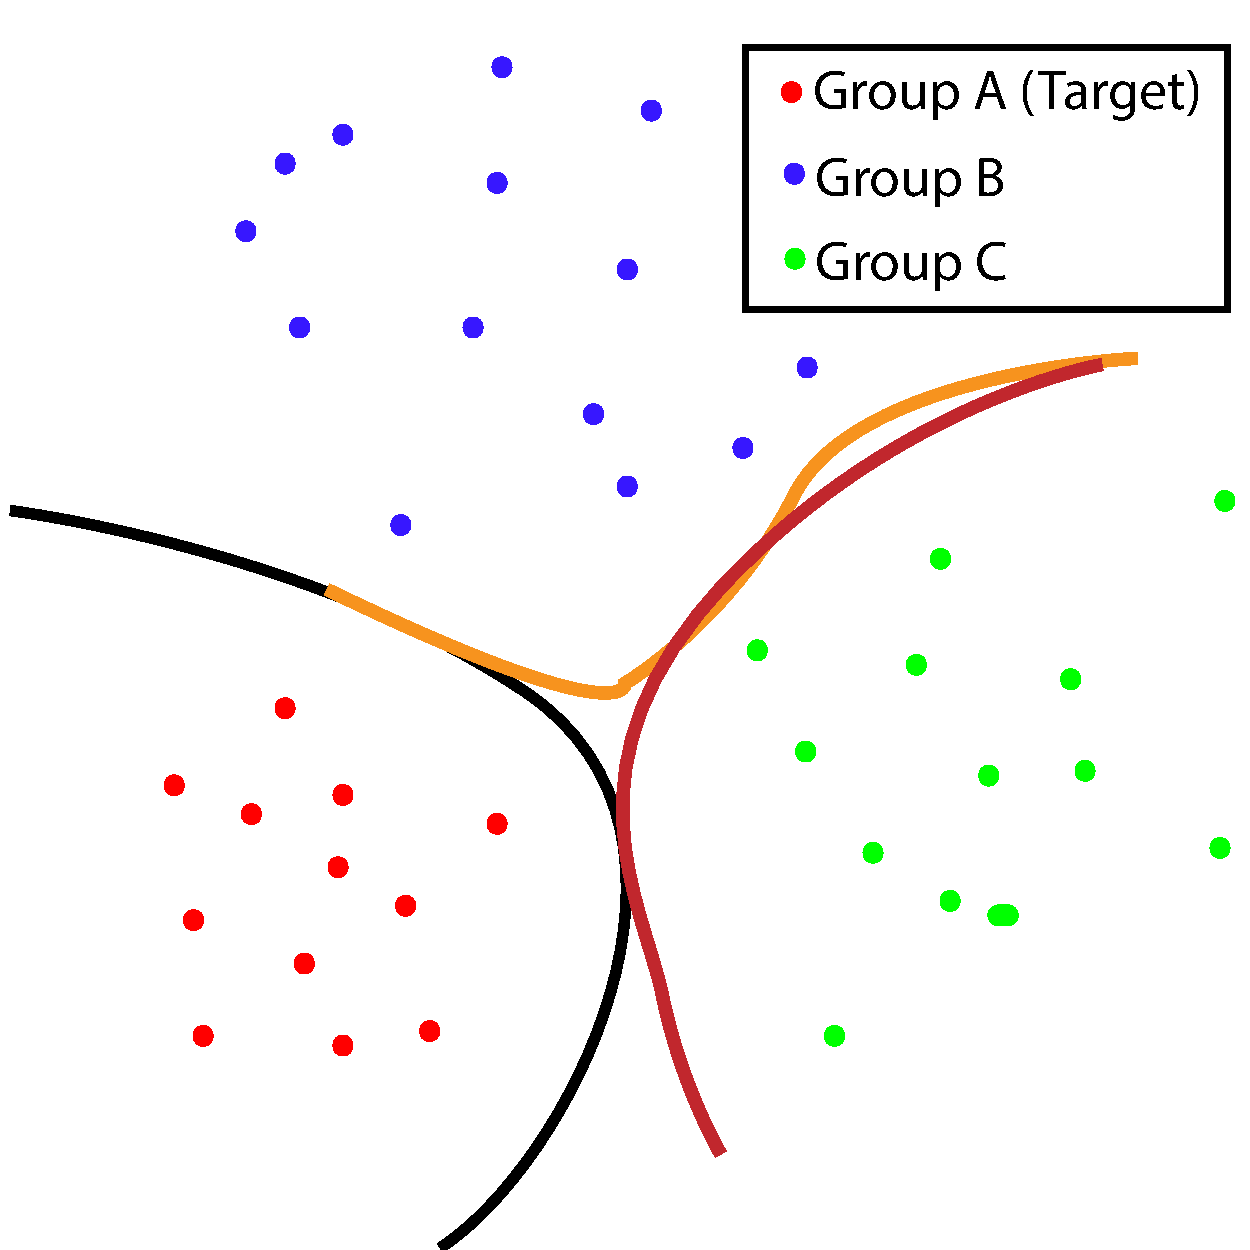
\includegraphics[width=2.7in, fbox]{Chapter2/1to1.pdf}
        \caption{One-to-one Multi-classification}
        \label{fig:121} 
    \end{subfigure}%
    ~
    \begin{subfigure}[b]{0.49\textwidth}
        \centering
        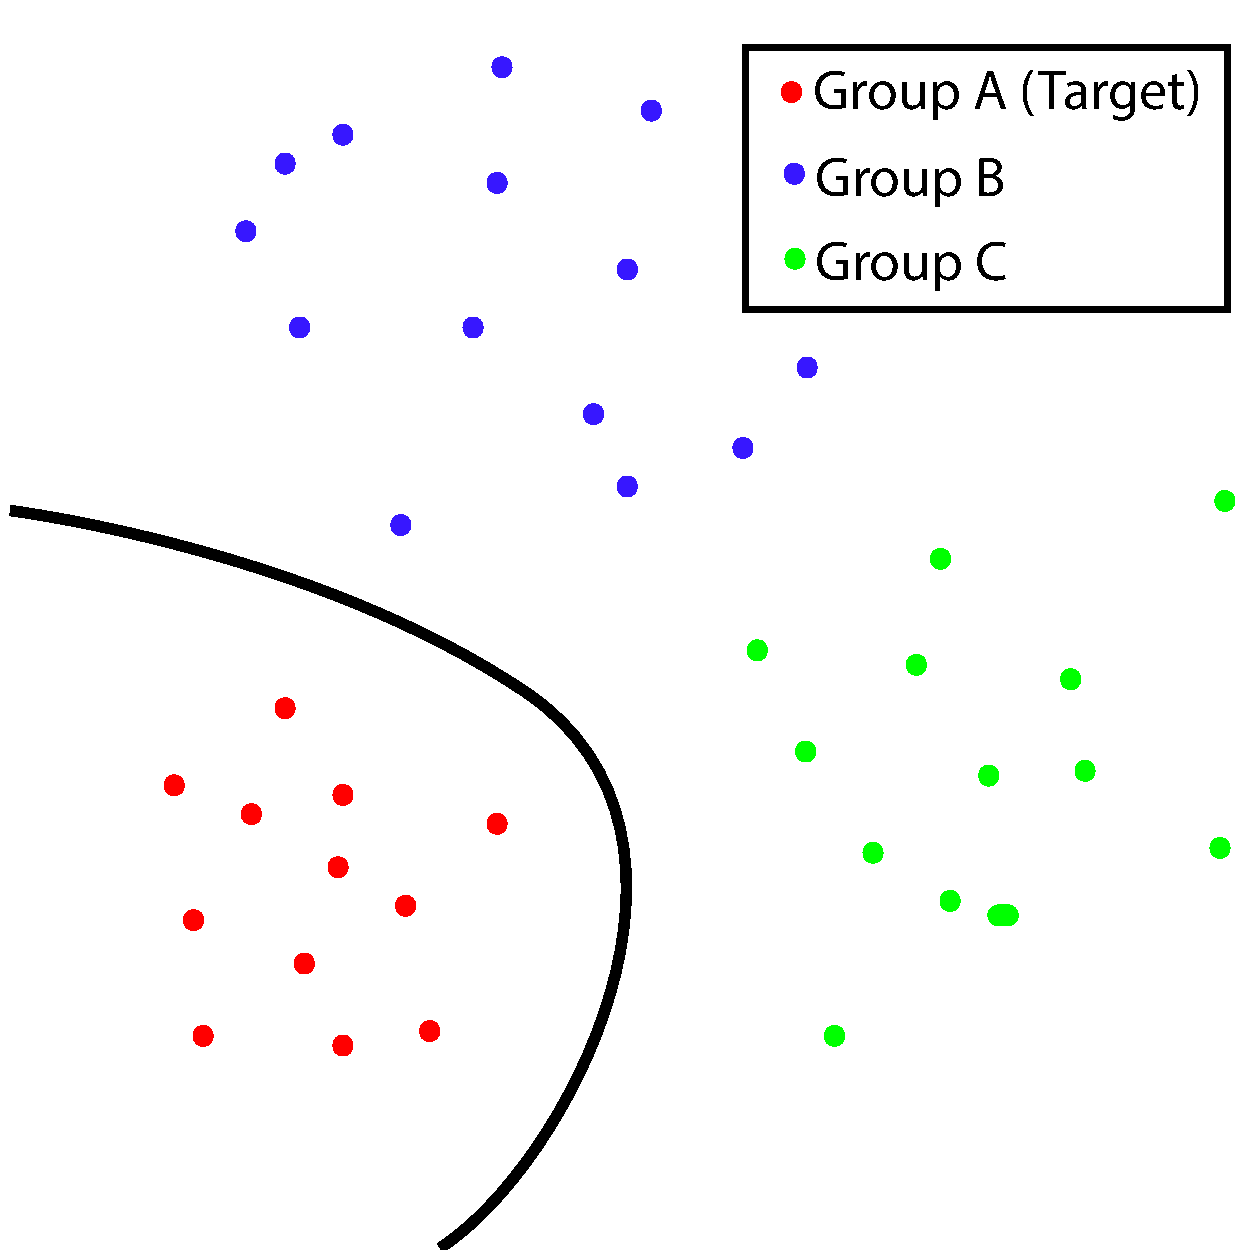
\includegraphics[width=2.7in, fbox]{Chapter2/1toall.pdf}
        \caption{One-to-all Multi-classification}
        \label{fig:12all} 
    \end{subfigure}
    \caption{Two Aggregated Algorithms}
\end{figure}


\subsection{Representation Learning and Deep Learning}

The main drawback of conventional machine-learning techniques is that they can not extract the features automatically and precisely from the raw input data. When using machine learning, engineers and researchers have to transform the raw data into normalized vectors that is suitable for training~\cite{ongsulee2017artificial}. Form the normalized vectors, the machine learning model can classify and do detection on the classify patterns.

Representation learning allows the machine to discover the best representation form of the raw data for machine learning training. Representation learning features that the algorithm can find and fit the best representation from the raw input data, no matter what format the input data is. Such representation of raw data is suitable for the further feature extraction~\cite{bengio2013representation}. For example, if the input is a gray-scale image, the output matrix after first representation layer would represent the position of edges and corners.

\begin{figure}[th]
    \centering
    \begin{subfigure}[b]{0.99\textwidth}
        \centering
        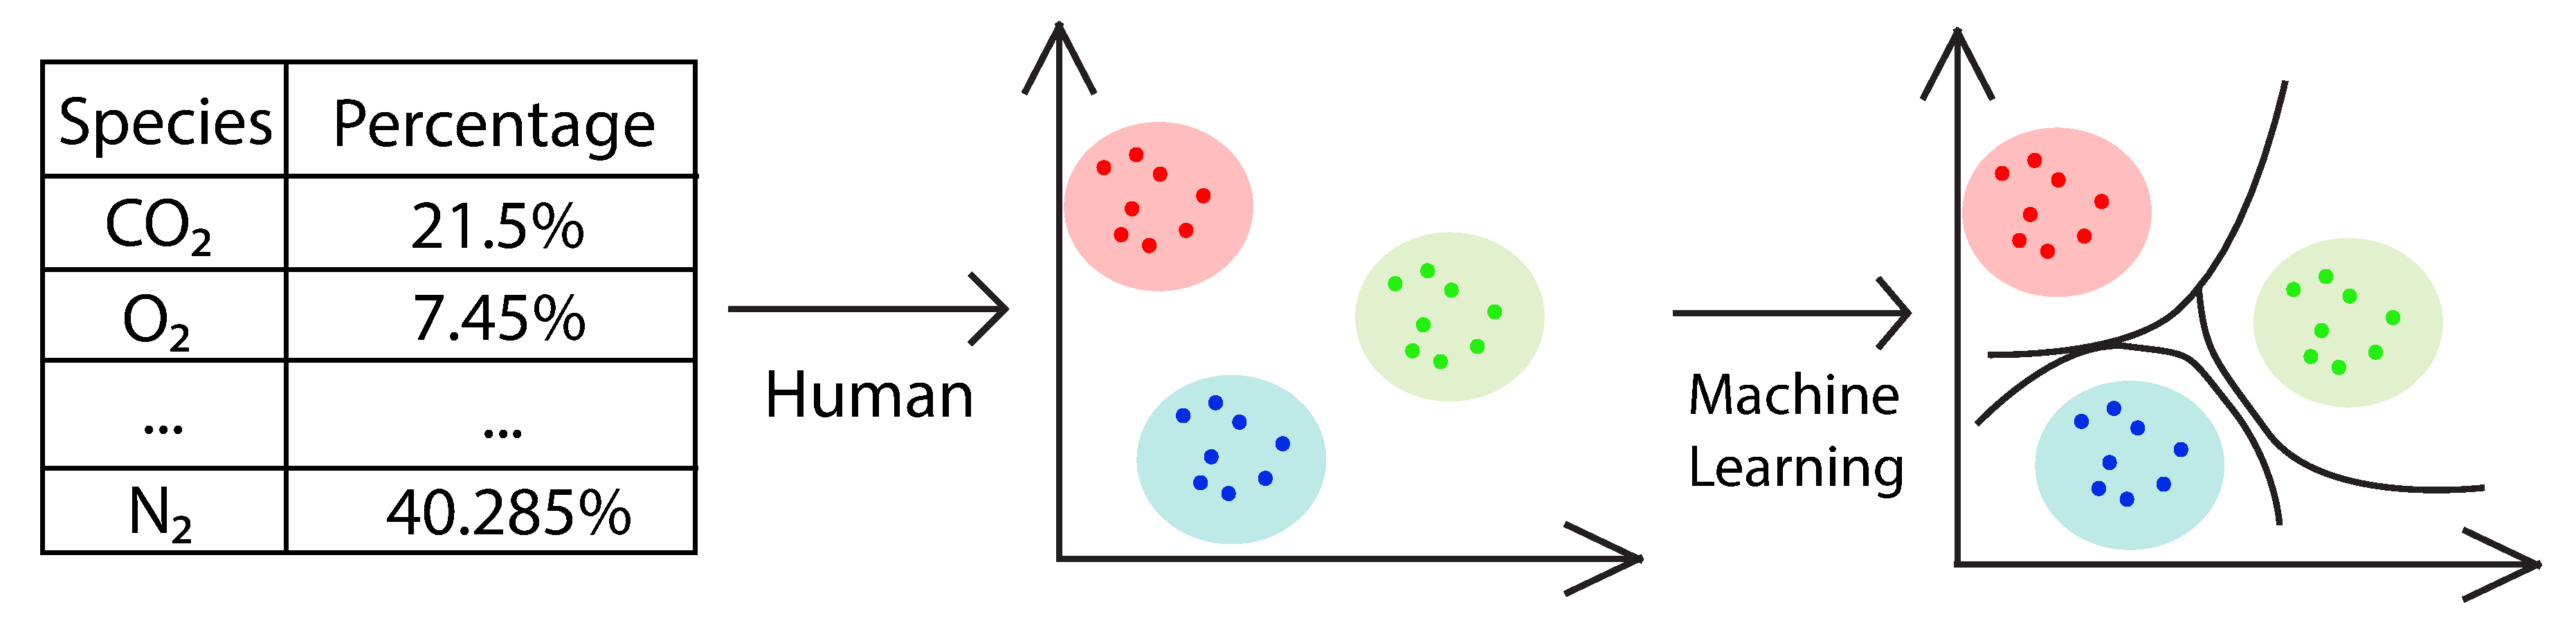
\includegraphics[width=0.98\textwidth, fbox]{Chapter2/Machine-Learing.pdf}
        \caption{Machine Learning: Human Data Centering}
        \label{fig:mldiagram} 
    \end{subfigure}%
    \\
    \begin{subfigure}[b]{0.99\textwidth}
        \centering
        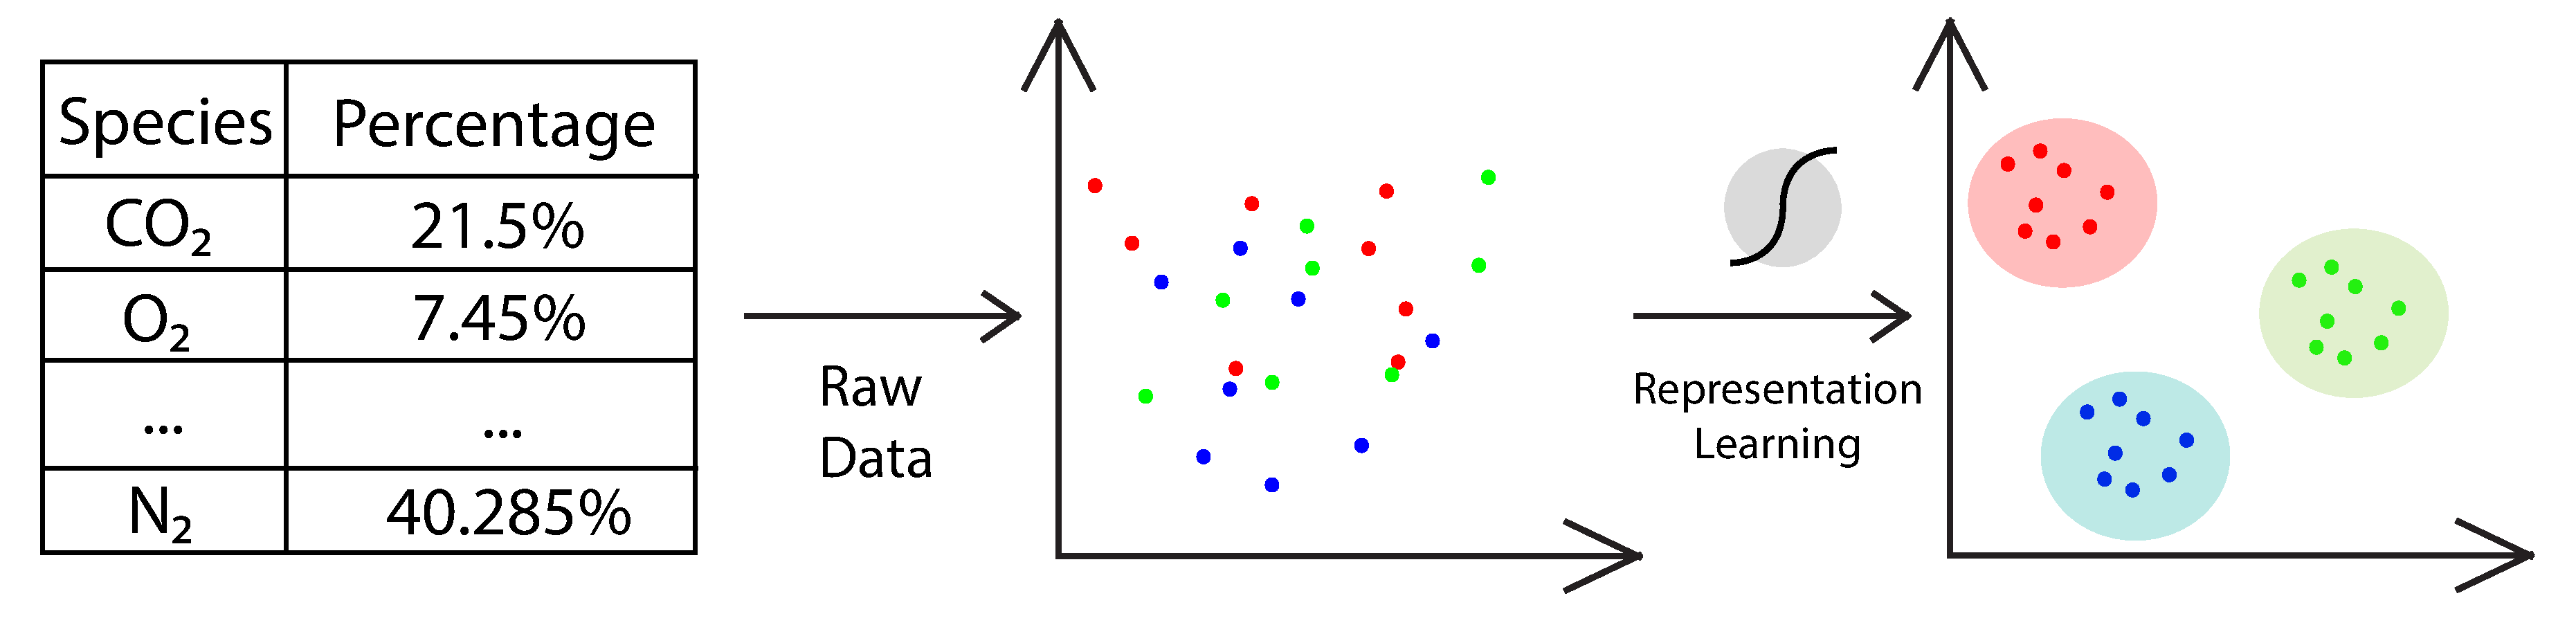
\includegraphics[width=0.98\textwidth, fbox]{Chapter2/Represent-Learing.pdf}
        \caption{Representation Learning: Auto Extraction}
        \label{fig:representdiagram} 
    \end{subfigure}
    \\
    \begin{subfigure}[b]{0.99\textwidth}
        \centering
        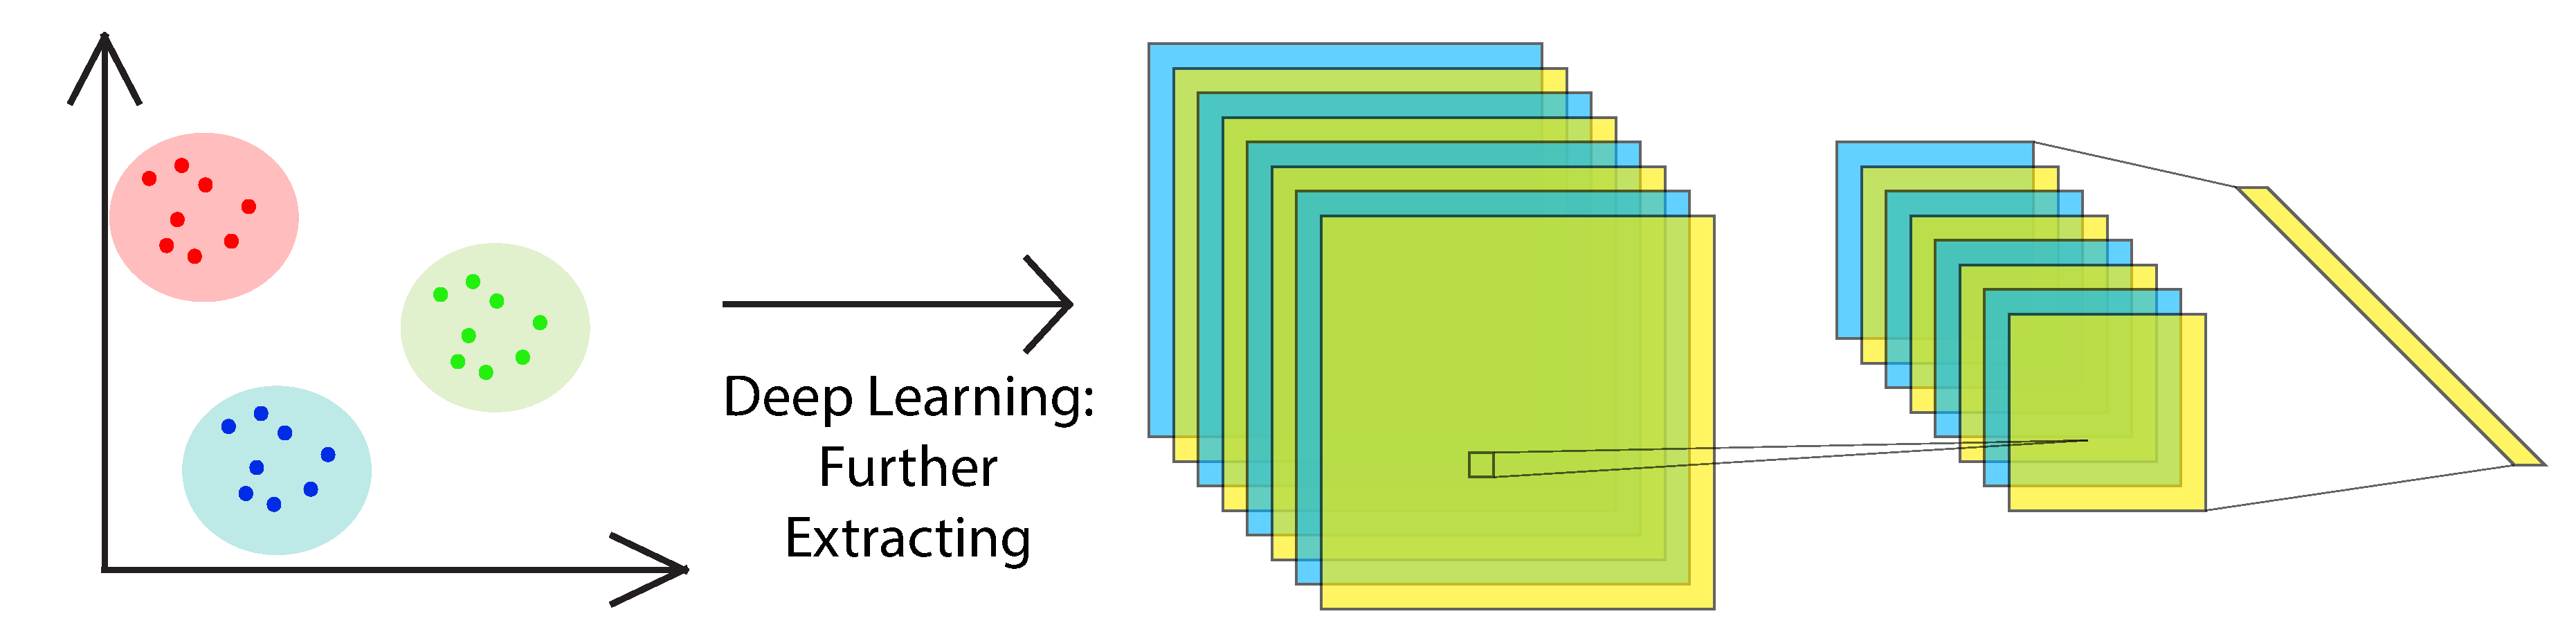
\includegraphics[width=0.98\textwidth, fbox]{Chapter2/Deep-Learing.pdf}
        \caption{Deep Learning: Further Extraction of Features}
        \label{fig:dldiagram} 
    \end{subfigure}%
    \caption{Comparison between Three Learning}
\end{figure}

Based on representation learning, the concept of deep learning was originally proposed in a study on Artificial Neural Network (ANNs) \cite{hinton2006reducing}. Basically, deep learning is a multi-layer and deeper version of representation learning. Deep learning can not only extract the features vectors from the first layer but also can go deeper, get more abstract high-level features. For example, if the input is a gray-scale image, the first layer of deep learning is just like the representation learning, extracting the position of edges and corners. The second layer of deep learning would extract the relative positions between the edges and corners, and the third layer of deep learning would treat edges and corners in similar shape as a group. With the network go deeper, such high-level abstract features can be sensed. In 2006, with a deep learning architecture called deep belief network (DBN) \cite{hinton2006fast} being invented by Hinton, the machine learning community rekindled heated discussion over deep-learning.

Give an example to illustrate the difference between the machine learning, representation learning and deep learning. For a chemical substances classification task, the input is the percentage of each components in a chemical mixture. When using machine learning algorithms like SVM, researchers have to re-form and normalize the input data, into a sparse data space, and should do multi-phase training for multi-classification (\autoref{fig:mldiagram}). When using representation learning methods, the input data can be raw data that has not been pre-processed (\autoref{fig:representdiagram}), such raw data will be mapped to high-dimension space by non-linear neural units. When using deep learning, the extracting layer goes deeper, thus can get more abstract features (\autoref{fig:dldiagram}).

Deep learning~\cite{lecun2015deep} is composed by simple non-linear \textit{Neural Unit} in each level. \textit{Neural Unit} is described in \autoref{subsec:neural_unit}. Deep learning uses the back propagation and feedforward mechanism to optimize the non-linear parameters of \textit{Neural Unit} from front to end. Propagation and feedforwad are described in \autoref{subsec:back_propagation}.


\subsection{Supervised, Unsupervised and Reinforcement Learning}

Machine learning algorithms can be classified into three main categories, according to the training data form and the learning mechanism of the algorithm: the supervised learning, the unsupervised learning and the reinforcement learning \cite{mohri2018foundations}. Between supervised learning and unsupervised learning, there are also semi-supervised learning.

Supervised learning is trained on labeled input and output~\cite{sen2020supervised, kotsiantis2007supervised}. Each input data $D_i$ is paired with a label or ground-truth value $L_i$, thus the training data should be in the format: $(D_i, L_i), i \in \mathbb{Z}$. The supervised learning aims to predict the corresponding label $l_i$ for each new input $d_i$. Supervised learning can be divided into two types: 

\begin{enumerate}
    \item Regression, when the label set $\{L_i\} = \mathbb{R}$, in which $\mathbb{R}$ is continuous real number set.
    \item Classification, when the label set $\{L_i\} = \mathbb{A}$, in which $\mathbb{A}$ is a set of discrete values $\{\alpha_1, \alpha_2, ...\}$ representing different classes.
\end{enumerate}

Unsupervised learning is to cluster unlabeled data set into different groups according to their feature\cite{meena2019survey}. It analyzes the bounding of a given vector set $\{D_1, D_2, ...,D_n\}$ (the training data), divide the set into $n$ groups $\{G_1, G_2, ..., G_n\}$, and tell if a new unseen data $d_i$ belongs to or not belongs to certain class $G_i$.

\begin{figure}[ht]
\centering
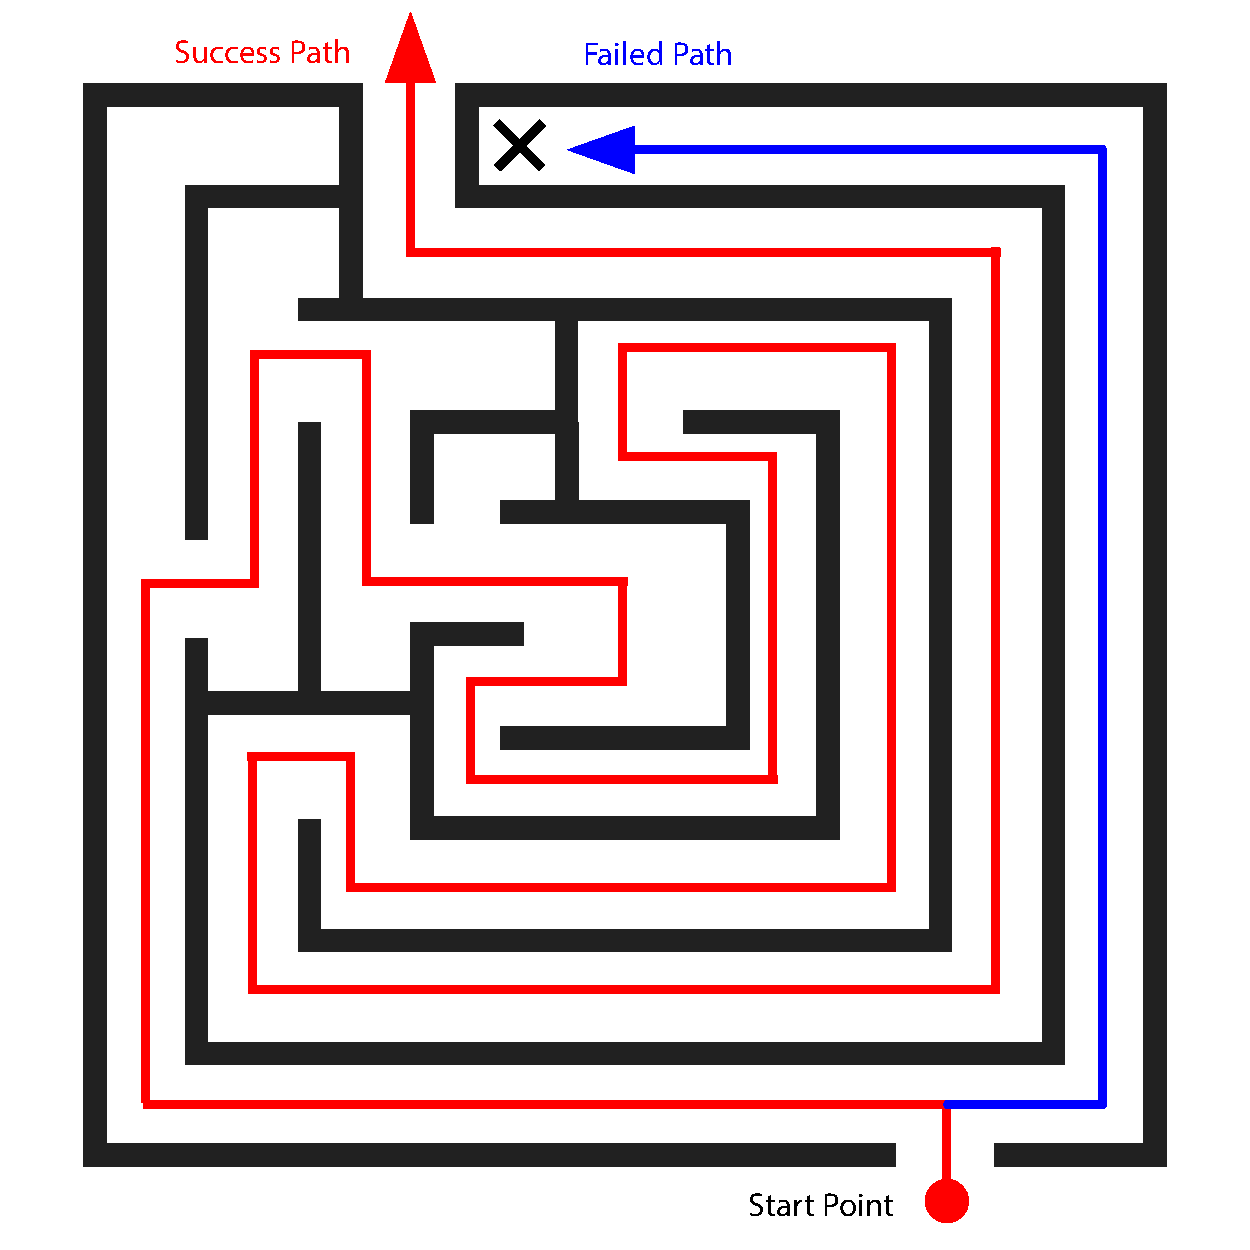
\includegraphics[width=0.75\textwidth, fbox]{Chapter2/reinforcement.pdf}
\caption{Reinforcement Learning: Maze Game Decisions}
\label{fig:reinforcement} 
\end{figure}

Reinforcement learning is to make the agent to play a game, or to perform a series of actions to reach to a certain goal~\cite{barto2004reinforcement}. The model will face a game-like situation, and make a consequence of decision to achieve the highest game score, as shown in~\autoref{fig:reinforcement}. First, the agent will observe the environment $\{\vec{E_i}\}$, which is a set of vectors representing the surrounding conditions. Second, the agent will conduct some action $\vec{a_i}$, and receive the reward/punishment score $\tau_i$. The aim of reinforcement learning is to find set of actions $\{\vec{a_i}\}, i \in (1,N)$, and such actions should satisfy the condition as described in~\autoref{eq:reinforce}.

\begin{equation}
\label{eq:reinforce}
   z = \argmax_{\{\vec{a_i}\}} \sum_{i=1}^{N} \tau_i
\end{equation}

Semi-supervised learning is to train the model on partially labelled data set~\cite{zhu2009introduction, zhu2005semi}. This method is a intermediate product of supervised learning and unsupervised learning. It addresses the problem that the fully labelled training data is hard to get, usually taking a lot of time to annotating all the data manually. If given a small set of labelled data set $\mathbb{D}_{label} = \{(D,L)\}$ along with a large set of unlabeled data set $\mathbb{D}_{unlabel} = \{D\}$, the semi-supervised learning can utilize the $\mathbb{D}_{label}$ to get the center of clusters, and utilize the $\mathbb{D}_{unlabel}$ to make the problem into a clustering problem.

\subsection{Neural Unit}
\label{subsec:neural_unit}

\begin{figure}[ht]
\centering
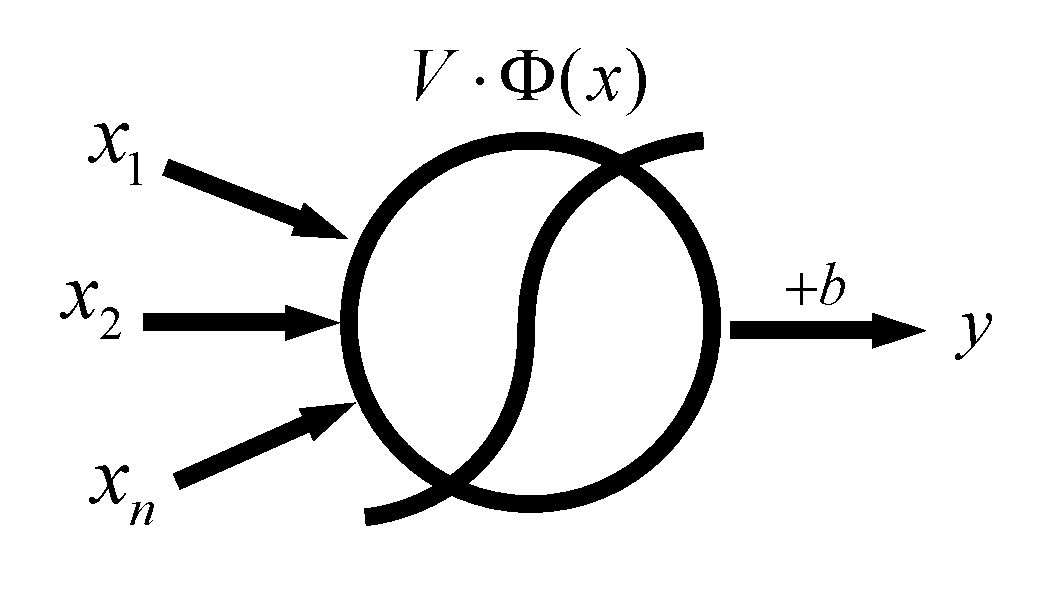
\includegraphics[width=0.5\textwidth, fbox]{Chapter2/neuralunit.pdf}
\caption{Neural Unit}
\label{fig:neuralunit} 
\end{figure}

The most basic unit that constructs the neural network is rather simple that is only a non-linear function with $n$ inputs and 1 output~\cite{bengio2017deep}, as shown in~\autoref{fig:neuralunit}. 

The function of input and output is as~\autoref{eq:neuralunit} shown. 

\begin{equation}
\label{eq:neuralunit}
    f(x)=b+V \cdot \Phi (c+W \vec{x})
\end{equation}

The $\Phi (\cdot)$ is the activation function, which could be some non-linear functions like \textit{Sigmoid} (\autoref{eq:sigmoid}), \textit{ReLU} (\autoref{eq:relu}) or \textit{Tanh} (\autoref{eq:tanh}). The image for the activation functions are shown in~\autoref{fig:activationfunc}. The activation function maps the input to another data space which is easier to perform classification. 

\begin{gather}
   \Phi_{Sigmoid}(x)=\frac{1}{1+e^{-x}} \label{eq:sigmoid}\\
   \Phi_{ReLu}(x)=max(0,x) \label{eq:relu}\\
   \Phi_{Tanh}(x)=tanh(x) \label{eq:tanh}
\end{gather}

\begin{figure}[th]
    \centering
    \begin{subfigure}[b]{0.49\textwidth}
        \centering
        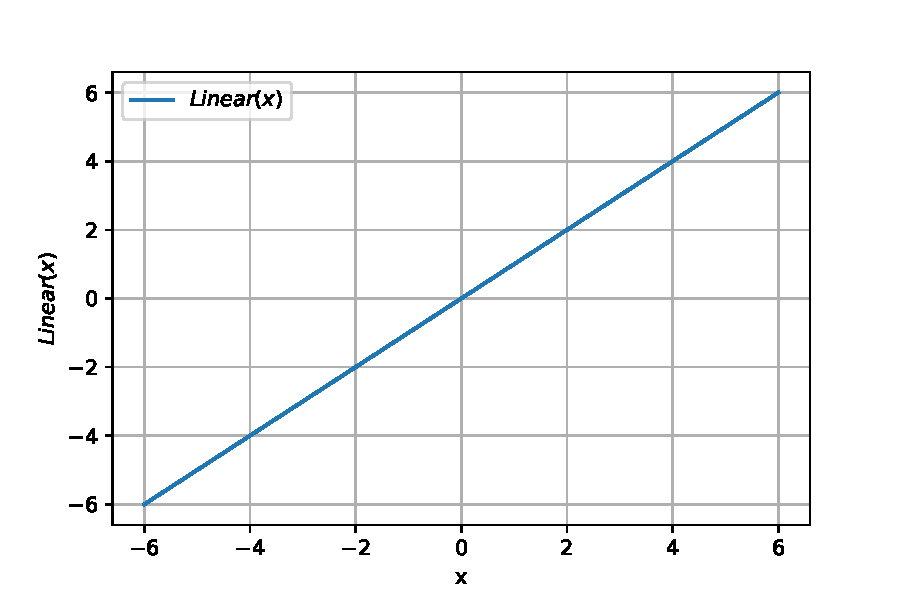
\includegraphics[width=2.7in, fbox]{Chapter2/linear.pdf}
        \caption{Linear}
    \end{subfigure}%
    ~
    \begin{subfigure}[b]{0.49\textwidth}
        \centering
        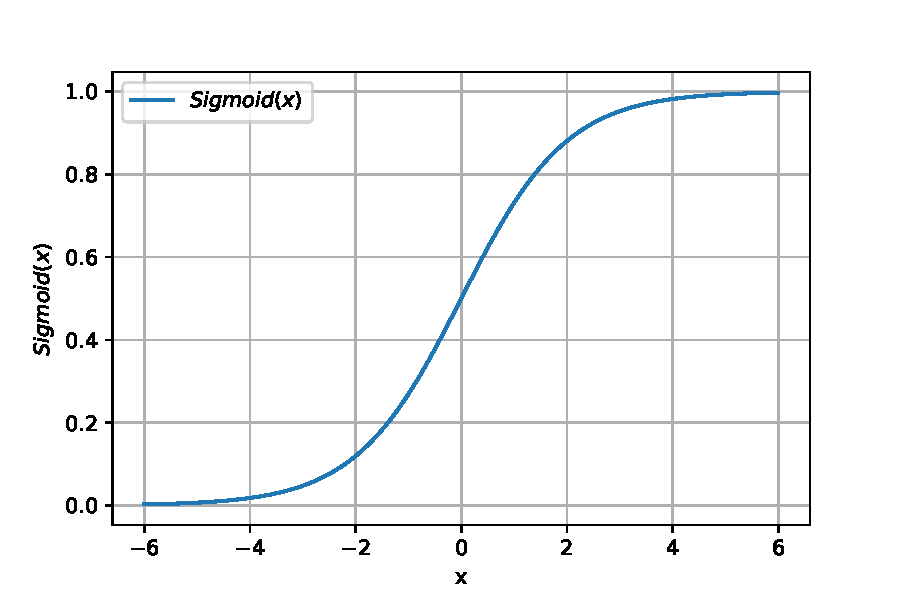
\includegraphics[width=2.7in, fbox]{Chapter2/sigmoid.pdf}
        \caption{Sigmoid}
        % \label{fig:sigfunc} 
    \end{subfigure}
    \\
    \begin{subfigure}[b]{0.49\textwidth}
        \centering
        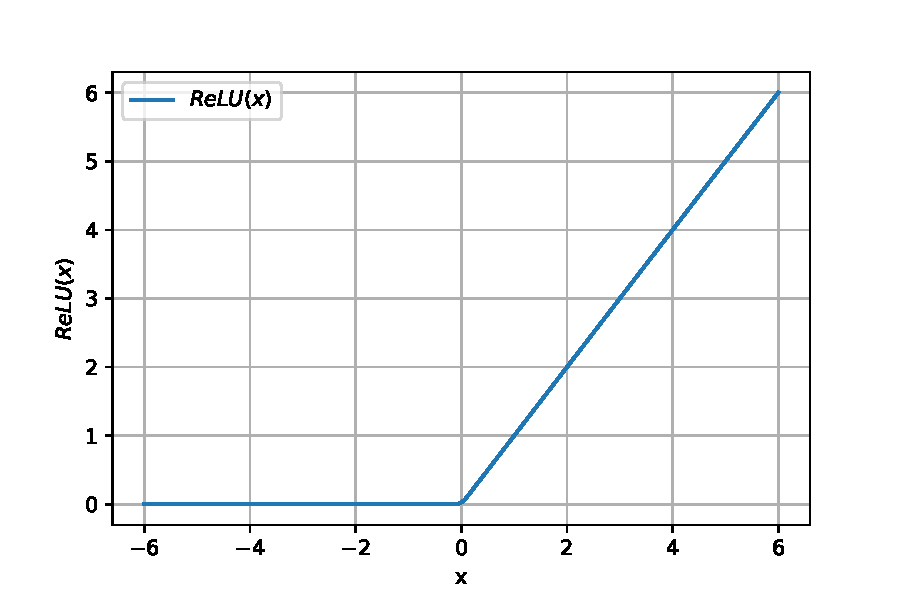
\includegraphics[width=2.7in, fbox]{Chapter2/ReLu.pdf}
        \caption{Rectified Linear Unit (ReLU)}
        % \label{fig:relufunc} 
    \end{subfigure}%
    ~
    \begin{subfigure}[b]{0.49\textwidth}
        \centering
        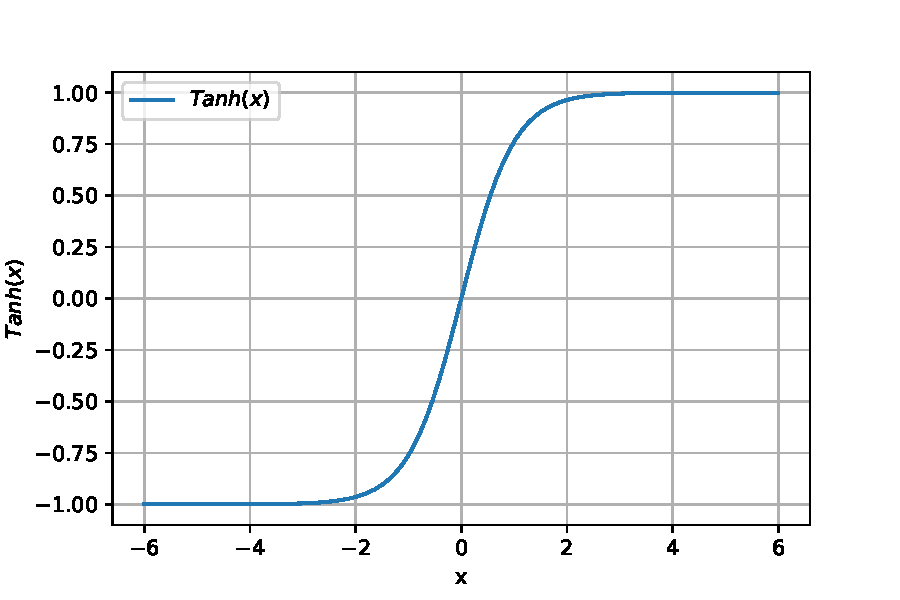
\includegraphics[width=2.7in, fbox]{Chapter2/tanh.pdf}
        \caption{Hyperbolic Tangent (Tanh)}
        \label{fig:tanhfunc} 
    \end{subfigure}
    \caption{Four Common Activation Functions}
    \label{fig:activationfunc} 
\end{figure}

For example, as shown in~\autoref{fig:activationlayer}, the blue line and red line in the input layer are the input data. The division line is a curve between the two classes. After the activation layer (\textit{Sigmoid} function), the 2-D input space is transformed into a 3-D shape so that the examples from two classes can be separated linearly (the black line in center image in~\autoref{fig:activationlayer} is the division line). The image is edited based on the Christopher Olah's origin version in  \href{http://colah.github.io/posts/2014-03-NN-Manifolds-Topology/}{http://colah.github.io}. The author has posted many insightful images, and these images are broadly used by Y.Lecun and Yoshua.B in their publications~\cite{bengio2017deep, lecun2015deep}. The $W_i$ is the weight of the $i$-th neural unit, which is the main parameter adjusted by back propagation process.


\begin{figure}[th]
\centering
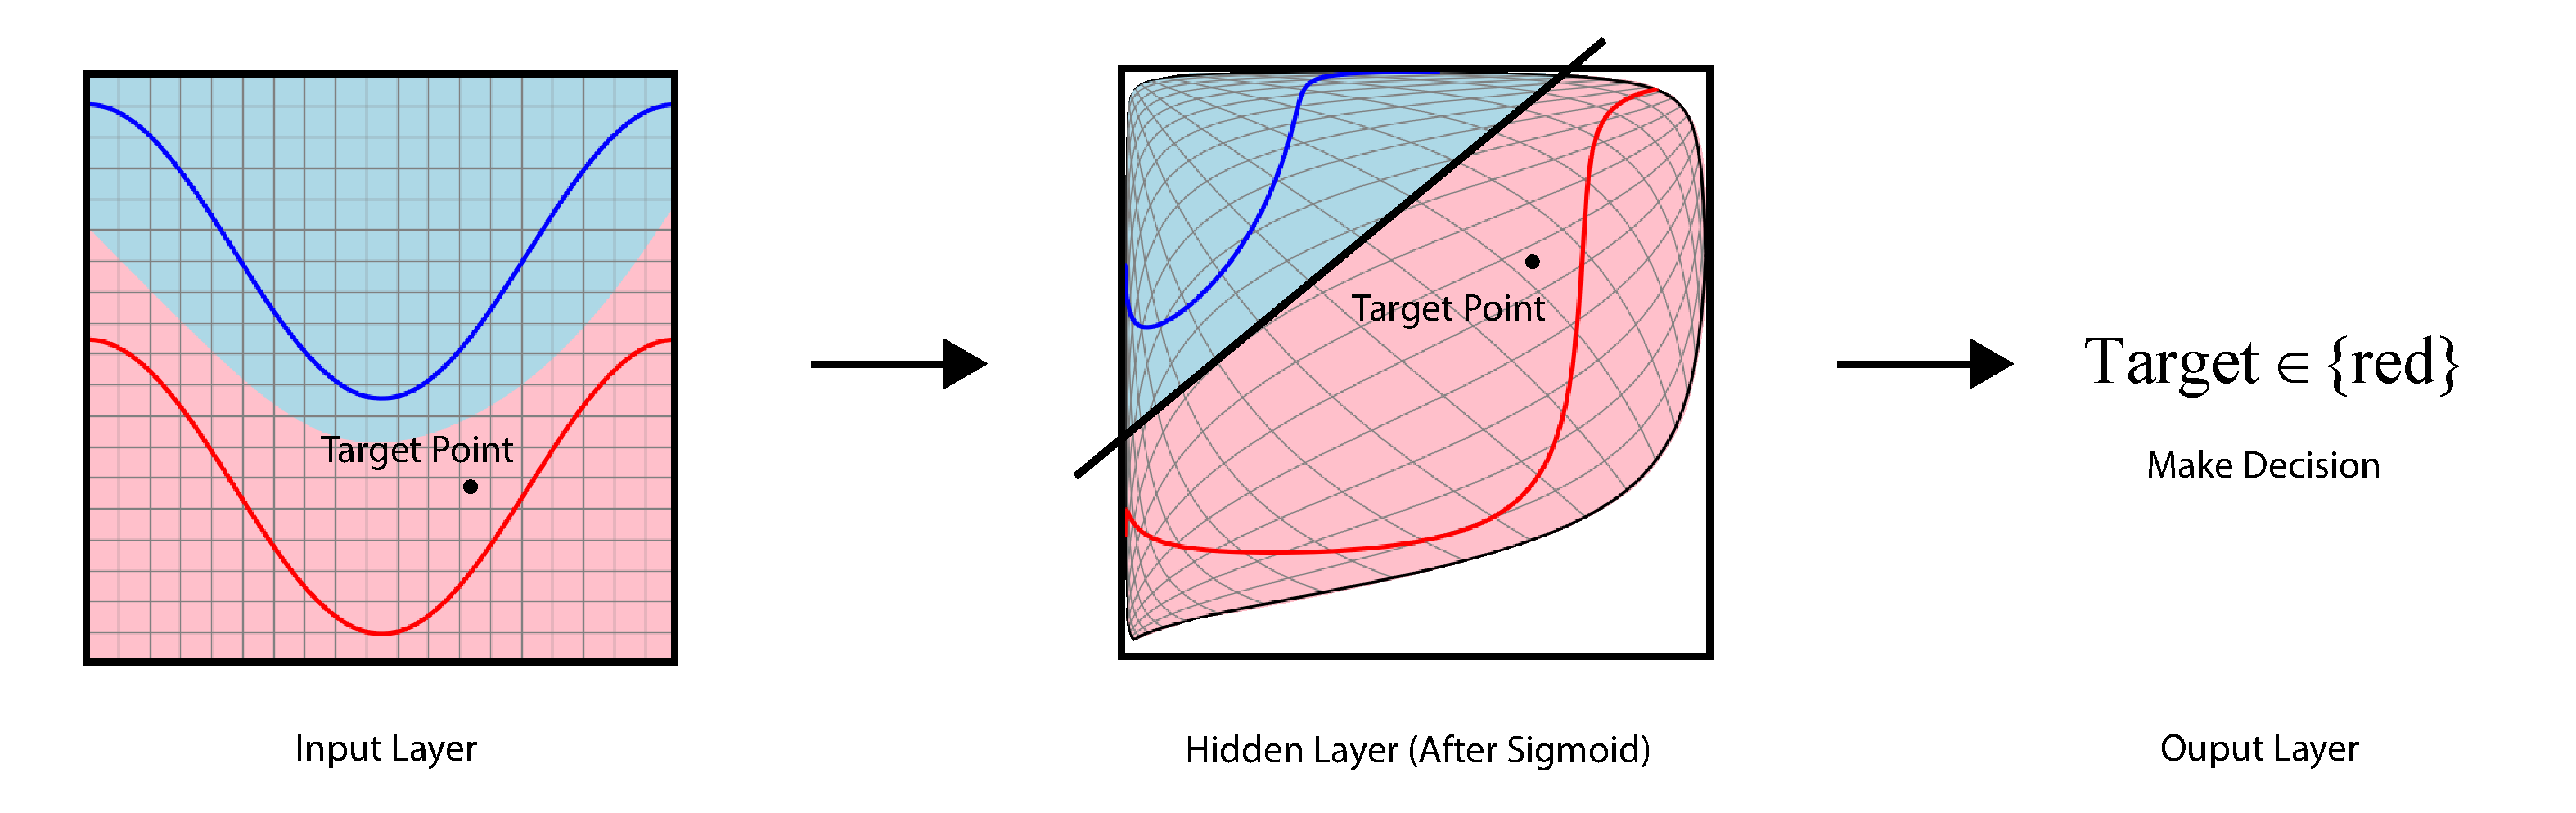
\includegraphics[width=0.99\textwidth, fbox]{Chapter2/activation.pdf}
\caption{Activation Kernal: Map to Nonlinear Data for Linear Decision~\cite{olah2014neural}}
\label{fig:activationlayer} 
\end{figure}

Any single layer in deep learning are made up by the non-linear neural units. As shown in~\autoref{fig:simplenn}, the input layer consists two neural units; the hidden layer (defined as those nodes not input either output), and it consists 9 nodes; the output layer consists only one node. Usually the output layer may consist of many nodes, in which case the \textit{flatten layer}, \textit{softmax layer} or other logistic regression functions are needed at the end of neural network, to make the output match with real-world case. And the parameter $W_i$, the weight of nodes, is the main part adjusted in the training process. This process is called feed-forward back propagation, which will be discussed in~\autoref{subsec:back_propagation}

\begin{figure}[th]
\centering
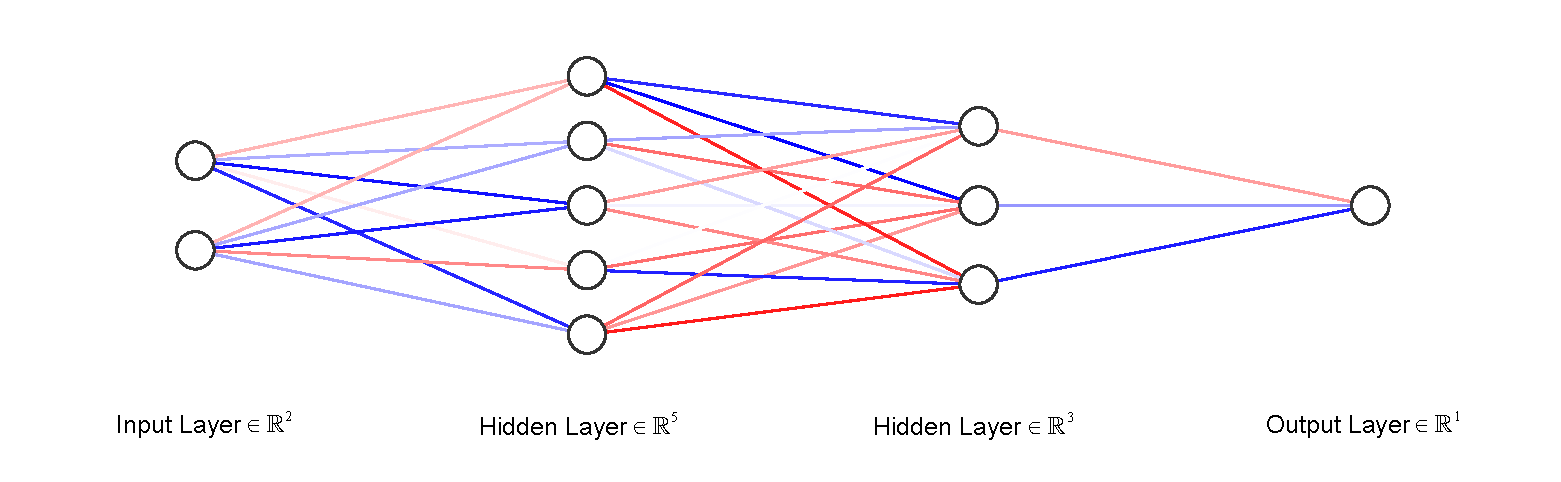
\includegraphics[width=0.99\textwidth, fbox]{Chapter2/simplenn.pdf}
\caption{Simple Neural Network}
\label{fig:simplenn} 
\end{figure}

\subsection{Back Propagation and Feedforward Network}
\label{subsec:back_propagation}

\subsection{Application}

GPT-3~\cite{brown2020language}

\section{Fully Convolution Networks}
\label{sec:LR_FCN}

\subsection{Convolutional Layer}

\subsection{Convolutional Neural Networks}

\section{Object Detection}
\label{sec:LR_objectdetection}



\section{Vanishing Points in Neural Networks}
\label{sec:LR_vpinNN}

\section{Concluding Remarks}

%=== END OF CHAPTER TWO ===
\end{spacing}
\newpage
